% Add "answers" option to print the answers
\documentclass[addpoints, answers]{exam}

\usepackage[utf8]{inputenc}
\usepackage{calc}
\usepackage[dvipsnames]{xcolor}
\usepackage{ifthen}
\usepackage{tcolorbox}

% \makebox[\textwidth]{Name:\enspace\hrulefill}
%  
% \vspace{5mm}
%\makebox[\textwidth]{Instructor’s name:\enspace\hrulefill}

\definecolor{MyLightGray}{gray}{0.60}

\newcommand{\truefalse}
{		\begin{checkboxes}
			 \choice True
			 \choice False. Explanation: 
		\end{checkboxes}
		\vspace{10pt}
}


% Check if 'answers' is an option
\newcommand{\ifanswers}[2]{%
  \ifthenelse{\boolean{exam@answers}}{#1}{#2}%
}



\newcommand{\answerspace}[1]
{
	\ifprintanswers
	\else
		\setlength{\mylength}{10pt}%
		% \vspace{#1\mylength}
		% Make the grey box
		\par\nobreak\noindent
		\makebox[\linewidth][l]{%
			% set inner padding to zero, so only the frame shows
			{\setlength{\fboxsep}{0pt}%
			% draw a color frame, white (or transparent) inside
			\fcolorbox{MyLightGray}{white}{%
			% the inner box has zero width content but fixed height
			\parbox[t][#1\mylength][c]{%
				% subtract twice the frame‐thickness from the full width
				\dimexpr\linewidth-2\fboxrule\relax
			}{\strut}%
			}%
			}%
		}%
		\par
		\vspace{3\mylength}

  	\fi
}
\newlength{\mylength}

\newcommand{\code}[1]{{\texttt{#1}}}

\newcommand{\answer}[1]{\begin{solution}{#1}\end{solution}}




%\usepackage{listings}
\usepackage{color}
\usepackage{lastpage}
\usepackage{verbatim}
\usepackage{fancyvrb}
\usepackage{graphicx}
\usepackage{float}
\usepackage{minted}
\usepackage{multicol}
\usepackage{amssymb}
\usepackage{amsmath}

\newcommand{\includecode}[2][c]{\lstinputlisting[caption=, escapechar=, language=#1]{#2}<!---->}
\RecustomVerbatimCommand{\VerbatimInput}{VerbatimInput}{}

\newcommand{\Code}[1]{\mintinline{java}{#1}}
\newcommand{\ACC}[4]{\{\Code{x}$\mapsto$\Code{#1},
  \Code{a}$\mapsto$\Code{#2}, \Code{b}$\mapsto$\Code{#3}, \Code{y}$\mapsto$\Code{#4}\}}

\renewcommand{\solutiontitle}{\noindent\textbf{Solution sketch: }}

\definecolor{SolutionColor}{rgb}{0.8,0.9,1}

\cfoot{Page \thepage\ of \pageref{LastPage}}

\rhead{Initials: \rule{20mm}{0.4pt}}



%%%%%%%%%%%%%%%%%%%%%%%%%%%%%%%%%%%%%%%%
\begin{document}
\fvset{numbers=left,numbersep=3pt}
\thispagestyle{empty}

\begin{center}
	{\LARGE CS 408 Spring 2026 -- Practice Final \\}

	\vspace{20mm}
\fbox{\fbox{\parbox{5.5in}{\centering
	\begin{itemize}
          % \item Write your \textbf{name} in the first page and your \textbf{initials in every other page}.
        \item The exam is closed notes, closed book.

        \item The exam should be completed individually: any
          communication with your fellow students is strictly
          prohibited.

	\item Please print or write legibly.

        \item If you have a question, raise your hand and the
          course staff will come to you.

        \item Provide complete and clear but concise
          answers. Any explanations should be thorough.

        \item Answer the questions in the spaces provided. Your answer
          does not need to take up all the space provided; if you run
          out of room, use the empty pages at the back of the exam to
          complete your answer.

        \item Coding questions should be answered in Java, unless
          requested otherwise.

        \item Unless otherwise noted, CFG nodes represent basic blocks.
          % or low-level pseudo-code.
          % \item Unless otherwise noted, assume that questions refer to C code, AT\&T assembly syntax and the x86 architecture.

        \item Please double check that your copy of the exam
          is complete; you should have \pageref{LastPage}
          pages.

        \item While the final will focus on content from the back half
          of the course (i.e., homeworks 3-5), the final is
          comprehensive, so everything we've covered is in scope.  You
          should be on top of everything from the midterm exam,
          though, so questions 8-15 are copies of the questions from
          the practice midterm to help you brush up on that earlier
          material.

        \item The questions we copied from the practice midterm all
          have 0 point values; we've otherwise assigned completely
          random points to questions 1-7, and you should not ascribe
          any meaning to those numbers.

        \item You will have 120 minutes to complete the actual final,
          but you can take as long as you need on this one :)
        \end{itemize}
	}}}
\end{center}

\vspace{5mm}
\begin{center}
  \resizebox{0.8\textwidth}{!}{
    \combinedgradetable[h][questions]
  }
\end{center}
%\begin{center}\combinedgradetable[h][questions]\end{center}
\vspace{5mm}


\makebox[\textwidth]{\textbf{Name (please print)}: \rule{100mm}{0.8pt} }
%\end{center}

\vspace{5mm}
%\begin{center}
\makebox[\textwidth]{\textbf{PUID}: \rule{40mm}{0.8pt} \hspace{35mm}}
%\end{center}


\begin{questions}

  \newpage


\question Consider the following predicate (call it $\phi$):
  \Code{(x <= a.length && !b) || x != y}
  \begin{parts}

\part[2] Write down the truth table for this predicate. %
  \answerspace{6} %
  \begin{solution}
    \begin{minipage}{.9\linewidth}
      \renewcommand{\arraystretch}{1.3}
      \begin{tabular}{|| c | c c c | p{1cm}||}
        \hline
        & \Code{x <= a.length} & \Code{b} & \Code{x != y} & $\phi$ \\ [0.5ex]
        \hline\hline
        1 & T & T & T & T \\   % h
        \hline
        2 & T & T & F & F \\   % g h i
        \hline
        3 & T & F & T & T \\
        \hline
        4 & T & F & F & T \\   % g h i
        \hline
        5 & F & T & T & T \\   % i
        \hline
        6 & F & T & F & F \\
        \hline
        7 & F & F & T & T \\   % g
        \hline
        8 & F & F & F & F \\   % g h i
        [1ex]
        \hline
      \end{tabular}
\end{minipage}
\end{solution}

\part[1] Provide a minimal set of test inputs to \Code{x}, \Code{a},
  \Code{b}, and \Code{y} that satisfy predicate coverage for
  $\phi$. If this is not possible, explain why. %
  \answerspace{6} %
  \begin{solution}
    Example Solution: \\
    \{\ACC{3}{[1,2,3,4]}{true}{4}, \\
    \ACC{3}{[1,2,3,4]}{true}{3}
    \}
  \end{solution}

% clause = basic elements (i.e., without logic ops)
\part[2] Provide a minimal set of test inputs to \Code{x}, \Code{a},
  \Code{b}, and \Code{y} that satisfy clause coverage for $\phi$. If
  this is not possible, explain why.
  \answerspace{5} %
  \begin{solution}
    Example Solution: \\
    \{\ACC{3}{[1,2,3,4]}{true}{4}, \\
    \ACC{10}{[1,2,3,4]}{false}{10}
    \}
\end{solution}

    % Steps:
    % p_a = (true ^ ~b) v c \xor (false ^ ~b) v c
    %     =    ~b v c       \xor  c, with x \xor y = (x and ~y) or (~x and y)
    %     =  ( (~b v c) ^ ~c ) or (~(~b v c) ^ c)
    %     =         ~b ^ ~c    or 0
    %     = ~b ^ ~c
\part[3] Provide the fully simplified $\phi_\texttt{x <= a.length}$
  condition. You do not need to show simplification steps. %
  \answerspace{4} %
  \begin{solution}
    \Code{!b && x == y}
    % $\lnot b \land \lnot c$
  \end{solution}

    % p_b = (a ^ ~true) v c \xor (a ^ ~false) v c
    %     =           c     \xor  a v c
    %     = ( c ^ ~(a v c) ) v ( ~c ^ (a v c))
    %     =  c ^ (~a ^ ~c)   v (~c ^ a) v (~c ^ c)
    %     =          0       v (~c ^ a)
    %     = ~c ^ a
\part[3] Provide the final (simplified) $p_b$ condition without the
  simplification steps. %
  \answerspace{4} %
  \begin{solution}
    \Code{x <= a.length && x == y}
    %$a \land \lnot c$
  \end{solution}

    % p_c = (a ^ ~b) v true \xor (a ^ ~b) v false
    %     =        true     \xor (a ^ ~b)           , 1 \xor x = ~x
    %     = ~(a ^ ~b)
    %     = ~a v b
\part[3] Provide the final (simplified) $p_\texttt{x!=y}$ condition
  without the simplification steps. %
  \answerspace{4} %
  \begin{solution}
    \Code{!(x <= a.length) || b}
    %$\lnot a \lor b$
  \end{solution}

    % minor c must be same when major c is true and s false
\part[4] Provide a minimal set of test inputs to \Code{x}, \Code{a},
  \Code{b}, and \Code{y} that satisfy Restricted Active Clause
  Coverage (RACC) for $\phi$. If this is not possible, explain why. %
  \answerspace{11} %
  \begin{solution}
    Example: \{ \\
    % \{a=T, b=F, c=F\}, % (a,b), P=T
    \ACC{0}{[1,2]}{false}{0}, \\
    % \{a=F, b=F, c=F\}, % (a,c), P=F
    \ACC{2}{[2]}{false}{2}, \\
    % \{a=F, b=F, c=T\}, % (c), P=T
    \ACC{2}{[1]}{false}{1}, \\
    % \{a=T, b=T, c=F\}  % (b), P=F
    \ACC{0}{[1,2]}{true}{0}
    \}
  \end{solution}

\part[4] Provide a minimal set of test inputs to \Code{x}, \Code{a},
  \Code{b}, and \Code{y} that satisfy Correlated Active Clause
  Coverage (CACC) for $\phi$. If this is not possible, explain why. %
  \answerspace{11} %
    \begin{solution}
      Example: \{ \\
      % \{a=T, b=T, c=F\},  % (a, b), P=T
      \ACC{0}{[1,2]}{false}{0}, \\
      % \{a=T, b=F, c=F\},  % (b)   , P=F
      \ACC{2}{[3,5,6]}{true}{2}, \\
      % \{a=F, b=T, c=F\},  % (a, c), P=F
      \ACC{3}{[1,2]}{false}{3}, \\
      %\{a=T, b=F, c=T\}   % (c), P=T
      \ACC{3}{[1,2,3,4]}{true}{4}
      \} \\
      \textbf{Note 1:} This test set does not satisfy RACC, because the two
      tests covering the case where where \Code{x !=y} determines
      $\phi$ do not have the same truth values for the other
      clauses.\\
      \textbf{Note 2:} We could also have used the answer from the
      previous question here. Why?
    \end{solution}

  \part[4] Provide a minimal set of test inputs to \Code{x}, \Code{a},
    \Code{b}, and \Code{y} that satisfy Generalized Active Clause
    Coverage (GACC) for $\phi$. If this is not possible, explain
    why. %
    \answerspace{11} %
    \begin{solution}
      Example: \{ \\
      % \{a=T, b=T, c=F\},  % (a, b), P=T
      \ACC{0}{[1,2]}{false}{0}, \\
      % \{a=F, b=T, c=F\},  % (a, c), P=F
      \ACC{2}{[1]}{false}{2}, \\
      % \{a=T, b=F, c=F\},  % (b), P=F
      \ACC{0}{[1,2]}{true}{0}, \\
      % \{a=F, b=T, c=T\}   % (c), P=T
      \ACC{3}{[1,2]}{false}{4}
      % \{a=F, b=F, c=T\}   % (c), P=T (repeated as g)
      %???
      \} \\
      \textbf{Note:} We cannot come up with a test set that satisfies
      GACC but not CACC here: in every scenario where \Code{x !=y}
      determines the value of $\phi$, $\phi$ has the same truth value
      as \Code{x !=y}: thus, any pair of tests from this test set
      which make \Code{x !=y} different values also cause $\phi$ to
      have different values.
    \end{solution}

\end{parts}

\newpage

\question[2] Suppose we have a predicate with $n$ clauses. What is the
  minimum number of elements a test set \textbf{must} contain in order
  to provide 100\% RACC for this predicate? What about for CACC and
  GACC? Explain your answer.  \answerspace{11} %
  \begin{solution}
    \begin{itemize}
      \item \textbf{RACC:} $n + 1$ \\
      \item \textbf{CACC:} 3 \\
        To show that given $n$ clauses, $c_1, c_2, \ldots, c_n$, it is
        possible to define a predicate where a set of at most 3 tests
        achieves 100\% CACC, consider a predicate of the form:
        \[
          c_1 \oplus c_2 \oplus \ldots \oplus c_n
        \]
        We'll define our test set in different ways, based on whether
        $n$ is odd or even. \\
        When $n$ is odd, we can use the following test set:
        \begin{itemize}
        \item [T1:] [$c_1 \mapsto$ \Code{true}, $\ldots$, $c_n \mapsto$ \Code{true}]
        \item [T2:] [$c_1 \mapsto$ \Code{false}, $\ldots$,
          $c_n \mapsto$ \Code{false}]
        \end{itemize}
        Observe that each $c_i$ is active in both tests: flipping the
        truth value of any $c_i$ in either test flips the value of
        $p$. Furthermore, the truth value assigned to each $c_i$ is
        different under T1 and T2. Finally, note that $c_1$ is acting
        as a parity bit for the other clauses, so $p$ is \Code{true}
        under T1 and \Code{false} under T2. Thus, this test achieves
        100\% CACC. \\
        When $n$ is even, we can use the following test set:
        \begin{itemize}
        \item [T1:] [$c_1 \mapsto$ \Code{true}, $\ldots$,
          $c_n \mapsto$ \Code{true}]
        \item [T2:] [$c_1 \mapsto$ \Code{true}, $c_2 \mapsto$
          \Code{false} $\ldots$, $c_n \mapsto$ \Code{false}]
        \item [T3:] [$c_1 \mapsto$ \Code{false}, $c_2 \mapsto$
          \Code{true} $\ldots$, $c_n \mapsto$ \Code{true}]
        \end{itemize}
        Observe that $c_1$ is active in tests T1 and T3, and the
        remaining $c_i$ are active in tests T1 and T2. Furthermore,
        the truth value assigned to $c_1$ is different under T1 and
        T3, and the truth values for $c_2$ to $c_n$ are different
        under tests T1 and T2.  Finally, $p$ is \Code{false} under T1
        and \Code{true} under T2 and T3. Thus, this test achieves
        100\% CACC.
        % 4\footnote{It may also be possible to do
        %   this in fewer than 4 tests, but I have not been able to do
        %   so yet.}  \\
        % Given $n$ clauses, $c_1, c_2, \ldots, c_n$, it is possible to
        % define a predicate where a set of 4 tests achieves 100\%
        % CACC. The predicate has the form:
        % \[
        %   (\lnot c_1 \lor (c_2 \land c_3 \land \ldots \land c_n)) \land
        %   ( c_1 \lor c_2 \lor c_3 \lor \ldots \lor c_n)
        % \]
        % And our test set is:
        % \begin{itemize}
        % \item [T1:] [$c_1 \mapsto$ \Code{true}, $\ldots$ $c_n \mapsto$ \Code{true}]
        % \item [T2:] [$c_1 \mapsto$ \Code{false}, $\ldots$ $c_n \mapsto$ \Code{false}]
        % \item [T3:] [$c_1 \mapsto$ \Code{false}, $c_2 \mapsto$
        %   \Code{true}, $c_3 \mapsto$ \Code{false}, $\ldots$ $c_n
        %   \mapsto$ \Code{false}]
        % \item [T4:] [$c_1 \mapsto$ \Code{true}, $c_2 \mapsto$
        %   \Code{false}, $c_3 \mapsto$ \Code{true}, $\ldots$ $c_n \mapsto$ \Code{true}]
        % \end{itemize}
        %   % Suppose we have n clauses, c_0, c_1, c_2, ..., c_n, and
        %   % define a predicate p = (c_0 => c_1 /\ c_2 /\ ... /\ c_n)
        %   % /\ (~c_0 => c_1 || c_2 || .. || c_n). We need four tests
        %   % to achieve 100 \% CACC on this set. The first one sets all
        %   % clauses to true. The second sets all clauses to false. The
        %   % third sets all but c_1 to false, and the fourth sets all
        %   % but c_1 to true. In the first test, each of c_1 to c_n
        %   % determine p, and make p true. In the second test, each of
        %   % c_1 to c_2 again determine p and make p false. In the
        %   % third test, c_0 determines p and makes p true. Finally, in
        %   % the fourth test, c_0 determines p and makes p false.
        % We'll use T1 and T2 as to provide correlated coverage for
        % clauses $c_2$ to $c_n$. Observe that $p$ evaluate to
        % \Code{true} under T1 and \Code{false} under T2, and that
        % furthermore flipping any of the truth values of $c_2$ to $c_n$
        % in either test changes the truth value of $p$, i.e., they
        % determine $p$.  Next, we'll use T3 and T4 as to provide
        % correlated coverage for $c_1$. Observe that $p$ evaluate to
        % \Code{true} under T3 and \Code{false} under T4, and that
        % furthermore flipping the value of $c_1$ in either test changes
        % the truth value of $p$, i.e., it determines $p$.
        % % Consider a scenario in which a
        % % predicate only evaluates to true under \textbf{exactly one}
        % % truth assignment to its clauses, so that flipping the
        % % assignment to \textbf{any} clause causes it to evaluate to
        % % false. An example of such a clause is one that consists of a
        % % conjunction of boolean variables: %
        % % \Code{x1 && x2 && ... && xn}.  When this happens, we only need
        % % two tests to achieve 100\% CACC (in the best case scenario,
        % % such test inputs will exist): a test that makes the predicate
        % % true, and a second which flips the truth value assigned to
        % % each predicate.
      \item \textbf{GACC:} 2 \\
        CACC subsumes GACC, so the minimum can't be more than 3. It
        also can't be less than two: for any given clause, we need at
        least two test cases in which the clause determines $p$: one
        in which the clause is \Code{true} and one in which the clause
        is \Code{false}. \\
        With that out of the way, observe that the first test set from
        the previous example gives us 100\% GACC, regardless of
        whether $n$ is even or odd: in the even case, $p$ evaluates to
        \Code{false} under both interpretations, but that's okay under GACC!

        % we can use the construction
        % from the previous example and the first test
        % construction from the

        % With that out of the way, we'll show that given $n$ clauses,
        % $c_1, c_2, \ldots, c_n$, it is possible to define a predicate
        % where a set of 2 tests achieves 100\% GACC. The predicate has
        % the form:
        % \[
        %   c_1 \oplus c_2 \oplus \ldots c_n
        % \]
        % And our test set is:
        % \begin{itemize}
        % \item [T1:] [$c_1 \mapsto$ \Code{true}, $c_2 \mapsto$
        %   \Code{false}, $\ldots$ $c_{n-1} \mapsto$ \Code{true},
        %   $c_n \mapsto$ \Code{false}]
        % \item [T1:] [$c_1 \mapsto$ \Code{false}, $c_2 \mapsto$
        %   \Code{true}, $\ldots$ $c_{n-1} \mapsto$ \Code{false},
        %   $c_n \mapsto$ \Code{true}]
        % \end{itemize}
        % The key idea here is that each $c_i$ is active in both tests:
        % flipping the truth value of any $c_i$ in either test flips the
        % value of $p$. Furthemore, the truth value assigned to each
        % $c_i$ is different under both tests.
      \end{itemize}
  \end{solution}

\newpage

\question The following code fragment implements a bubble sort by
  sorting in-place the integers contained in an input array,

\begin{minted}{Java}
public static void bubbleSort3(int[] arr) {
  if (arr.length < 3) return;
  for (int i = 0; i < 3 - 1; i++) {
    for (int j = 0; j < 3 - i - 1; j++) {
      if (arr[j] > arr[j + 1]) {
        int temp = arr[j];
        arr[j] = arr[j + 1];
        arr[j + 1] = temp;
      }
    }
  }
}
\end{minted}

  \begin{parts}
  \part[3] Provide three concrete test inputs for \Code{bubbleSort}
    which induce distinct test paths. For each test input, show the
    final path constraint that concolic execution would produce. Give
    your answer as a sequence of path conditions separated by $\land$,
    e.g., for the path conditions $P$, $Q$, and $R$, write
    $P \land Q \land R$.  When writing your path condition, assume the
    initial symbolic input has the form
    $arr \mapsto [x_0, x_1, \ldots, x_n]$, and write the symbolic
    value stored at index $k$ as $x_k$. You are allowed to drop
    clauses that are always true, e.g., $3 < 5 + 1$ from the path
    constraint, but otherwise you should not simplify it in any way.
    \answerspace{9} %
    \begin{solution} %
      \begin{enumerate}
        \item \begin{itemize}
          \item \textbf{Concrete Input:} $arr \mapsto$ \Code{[1, 2]}
          \item \textbf{Symbolic Input:} $arr \mapsto$ {[$x_0$, $x_1$]}
          \item \textbf{Final Path Condition:} $arr.length < 3$
          \end{itemize}
        \item \begin{itemize}
          \item \textbf{Concrete Input:} $arr \mapsto$ \Code{[1, 2, 3]}
          \item \textbf{Symbolic Input:} $arr \mapsto$ [$x_0$,
              $x_1$, $x_2$]
          \item \textbf{Final Path Condition:} $\lnot (arr.length < 3)
            \land \lnot (x_0 > x_1) \land \lnot(x_1 > x_2) \land \lnot
            (x_0 > x_1)$
          \end{itemize}
        \item \begin{itemize}
          \item \textbf{Concrete Input:} $arr \mapsto$ \Code{[3, 2, 1]}
          \item \textbf{Symbolic Input:} $arr \mapsto$ {[$x_0$,
              $x_1$, $x_2$]}
          \item \textbf{Final Path Condition:} $\lnot (arr.length < 3)
            \land (x_0 > x_1) \land (x_0 > x_2) \land  (x_1 > x_2)$
          \end{itemize}
        \end{enumerate}
  \end{solution}

\newpage

  \part[3] For each of your concrete test inputs, provide a next test
    input that a concolic execution might produce.
    \answerspace{9} %
    \begin{solution} %
      \begin{enumerate}
      \item $arr \mapsto$ \Code{[1, 2, 3]}
      \item $arr \mapsto$ \Code{[2, 1, 3]}
      \item $arr \mapsto$ \Code{[3, 1, 2]}
      \end{enumerate}
    \end{solution}
\end{parts}

\question[3] Identify three categories of test oracles that we have
  discussed in class, and list the relative strengths and weakness of
  each.
  \answerspace{9} %
  \begin{solution} %
    \begin{description}
    \item[implicit oracles]
      \begin{description}
      \item[Pros:] Broadly applicable, require no extra user input,
        easy to automatically test
      \item[Cons:] Weak correctness guarantees, decreasing
        effectiveness over time
      \end{description}
    \item[human oracle]
      \begin{description}
      \item[Pros:] Very flexible, can be applied when correctness is
        hard to specify (think UI)
      \item[Cons:] Expensive and slow, does not scale
      \end{description}
    \item[reference implementation]
      \begin{description}
      \item[Pros:] Strong correctness guarantees, amenable to
        automated testing, particularly for regression testing
      \item[Cons:] Requires a gold standard reference implementation,
        which may be costly to build or maintain
      \end{description}
    \item[Property-Based Oracle]
      \begin{description}
      \item[Pros:] More expressive than implicit oracles, but can
        still be automatically tested, does not require reference implementation
      \item[Cons:] User effort required to identify properties, can
        miss bugs, correctness properties may be hard to specify
      \end{description}
    \item[Metamorphic Testing]
      \begin{description}
      \item[Pros:] Can identify bugs when correctness is hard to
        specify, e.g., classifiers, LLMs, graphics software
      \item[Cons:] User effort required to identify relevant
        properties, correctness often cannot be expressed as a
        metamorphic relation
      \end{description}
    \end{description}
  \end{solution}

\question[5] Suppose we are fuzz testing a program and discover that the
  input string ``axbxcxd'' causes the system under test to
  crash. Suppose that the delta debugging algorithm outputs the string
  ``xx''. Can you hypothesize what sorts of input strings are
  triggering the failure? Using that hypothesis, can you explain how
  \Code{ddmin} went from the initial input to its final output by
  providing four intermediate it might test, two of which induce this
  failure and two of which do not? Your answer should list these
  strings in the order in which \Code{ddmin} generates them.
  \answerspace{9} %
  \begin{solution} %
    One reasonable hypothesis is that the failure is triggered by an
    input that contains at least two ``x''s. This hypothesis is
    certainly supported by the minimal failing input returned by
    \Code{ddmin}.  Here are four test cases that would lend further
    credence to this hypothesis (succeeding cases are written in
    \textcolor{green}{green}, failing test cases are written in
    \textcolor{red}{red}) \textcolor{red}{``axbx''},
    \textcolor{green}{``ax''}, \textcolor{green}{``axb''}, and
    \textcolor{red}{``axx''}.
  \end{solution}

\newpage

\question[2] What is the key difference between dynamic and static
  analyses? What are the relative strengths and weaknesses of the two
  kinds of techniques?
  \answerspace{9} %
  \begin{solution} %
    Static analyses reason about a program's behavior without
    executing it, while dynamic analyses run a program to test its
    behaviors.
    \begin{description}
    \item[Static Analyses:]
      \begin{description}
      \item[Pro:] Needs only source code, no need to write tests
      \item[Pro:] Sound analyses conservatively identify all
        violations of a particular class of properties-- no warnings
        mean no failures from that class
      \item[Con:] Reported warnings may contain false positives
      \item[Con:] May not scale to large programs
      \end{description}
    \item[Dynamic Analyses:]
      \begin{description}
      \item[Pro:] Do not need access to source code
      \item[Pro:] Only real failures are reported-- if the test fails,
        the program has a problem
      \item[Pro:] Naturally scales to large or complex systems
      \item[Con:] Have to generate tests somehow
      \item[Con:] Can easily miss faults
      \end{description}
    \end{description}
  \end{solution}

\question The next two questions will ask you to give the annotated
  CFG that results from analyzing the program using the
  path-insensitive, forward data-flow analysis algorithm discussed in
  class.
\begin{minted}{Java}
  if (n == 42) {
    x = 2;
  } else {
    x = 0
  }
  while (x < n) {
    x = x + 2;
  }
  return x;
\end{minted}
  Each part gives you the Hasse diagram for the domain you should use
  in your anaylsis, and you should use %
  \mintinline{java}{[n } $\mapsto \top, $%
  \mintinline{java}{x} $\mapsto \bot$ \mintinline{java}{]} for the
  input abstract state for each question. Your answer should be given
  in the form of a CFG, where each node of the CFG is annotated with
  an input abstract state, basic block / conditional identifier, and
  an output abstract state. %

  \begin{parts}
  \part[3] Analyze this program using the following domain: \\ %

    \begin{minipage}{.25\linewidth}
      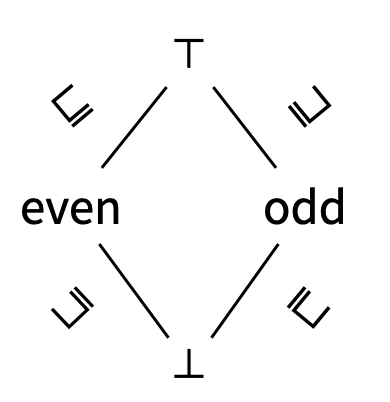
\includegraphics[width=\linewidth]{EvenOdd.png}
    \end{minipage}
    \begin{itemize}
      \item even: Even numbers $\equiv \{ n \in \mathbb{Z} ~|~ n~\%~ 2 = 0\}$
      \item odd: Odd numbers $\equiv \{ n \in \mathbb{Z} ~|~ n~\%~ 2 = 1\}$
      \item $\top$: All integers $\equiv \mathbb{Z}$
      \item $\bot$: Undefined $\equiv \emptyset$
      \end{itemize}

    Intuitively, this domain tracks if each variable is even, odd, or
    could be either even or odd. %
    \answerspace{9} %
    \begin{solution} %
      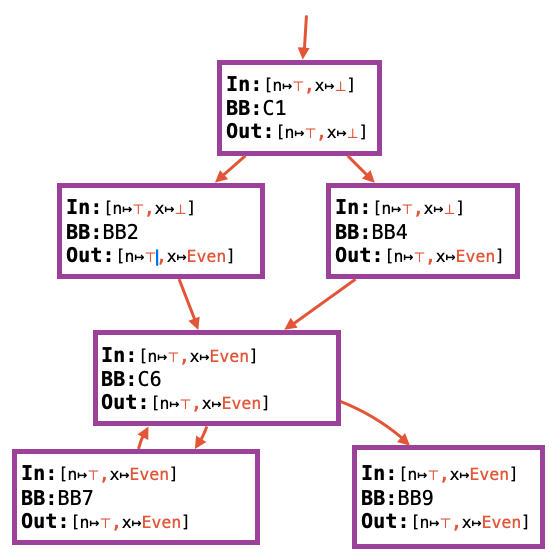
\includegraphics[width=.5\linewidth]{EvenOddCFG.png}
    \end{solution}

  \part[3] Analyze this program using the enhanced sign domain from
    class: \\
    \begin{minipage}{.25\linewidth}
      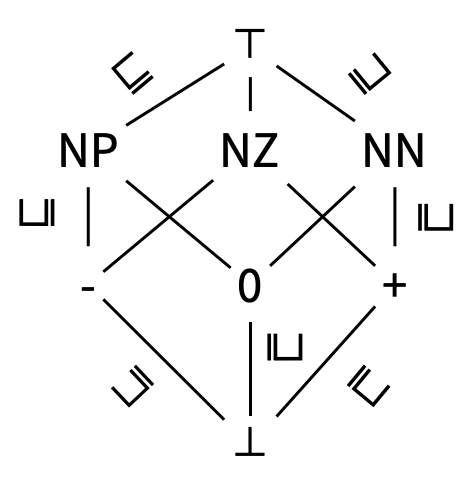
\includegraphics[width=\linewidth]{EnhancedSign.png}
    \end{minipage}
    \begin{itemize}
      \item +: Strictly positive $\equiv \{ n \in \mathbb{Z} ~|~ n > 0\}$
      \item -: Strictly negative $\equiv \{ n \in \mathbb{Z} ~|~ n < 0\}$
      \item 0: Zero $\equiv \{ 0\}$
      \item $\top$: All integers $\equiv \mathbb{Z}$
      \item $\bot$: Undefined $\equiv \emptyset$
      \item NN: Non-negative $\equiv \{ n \in \mathbb{Z} ~|~ 0 \leq n\}$
      \item NP: Non-positive $\equiv \{ n \in \mathbb{Z} ~|~ n \leq 0\}$
      \item NZ: Non-zero $\equiv \{ n \in \mathbb{Z} ~|~ n \neq 0 \}$
    \end{itemize}

    In addition to tracking whether each variable is positive,
    negative, zero, or any number, like the 'regular' sign domain,
    this domain tracks if a variable can be non-negative,
    non-positive, or non-zero. %
    \answerspace{9} %
    \begin{solution} %
      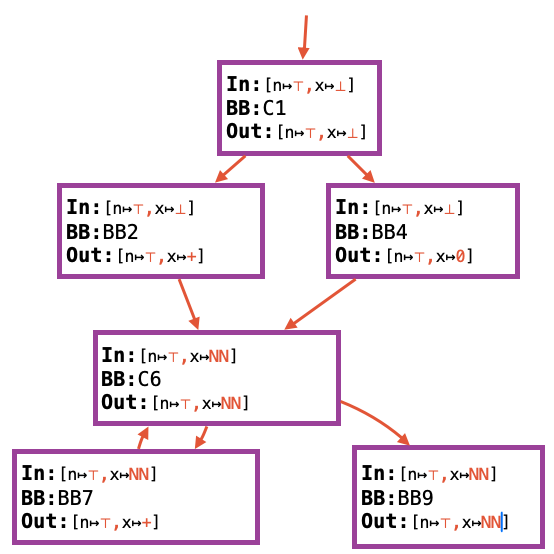
\includegraphics[width=.5\linewidth]{EnhancedSignCFG.png}
    \end{solution}

\newpage

  \part[1] How would your answer to the previous question change if
    you used the regular sign domain (discussed in class), which only
    tracks whether a variable is positive, negative, zero, or any
    number? %
    \answerspace{9} %
    \begin{solution} %
      The input/output value of x in most of the nodes would become
      $\top$, starting with the node that follows the two branches. In
      short, this domain is too coarse grained to capture the concept
      that a variable can be non-negative.
    \end{solution}

  \part[1] Suggest a simple tweak to the original program that would
    cause the data-flow analysis using the enhanced sign domain and
    the regular sign domain to have the same output CFG. %
    \answerspace{9} %
    \begin{solution} %
      Replace the assignment at line 4 with \Code{x = 4}; both domains
      are able to capture the fact that a variable is a positive number!
    \end{solution}
\end{parts}

\newpage

\question Consider the concept of faults, errors and failures.
  \begin{parts}

\part What is the difference between an error state and a failure?
  Explain. %
  \answerspace{9} %
  \begin{solution} %
    An error state is an \textit{incorrect internal state of the
      program}, e.g., when an internal variable holds a value it would
    never hold if the program did not conatin a fault.

    A failure is an observable behavior that is inconsistent
    with respect to the expected behavior: the program crashes
    when it should not, or it produces the wrong output).  %
  \end{solution}

\part What is the relationship between an error state and a
  failure? Explain. %
  \answerspace{10} %
  \begin{solution} %
    A program \textbf{must} encounter an error state in order for a
    failure to happenx, i.e., an error state is a \textit{necessary
      precondition} for a failure.

    Importantly, however, not all error states lead to failures.  %
  \end{solution}

\end{parts}

\question Consider the following three approaches to testing a function:
  \begin{itemize}
  \item \textbf{Approach 1:} Run the target program on $N$
    randomly chosen inputs
  \item \textbf{Approach 2:} Run the target program on a
    representative set of $N$ inputs
  \item \textbf{Approach 3:} Run the target program on all inputs
  \end{itemize}

  You can assume N is in the order of tens of thousands.

\begin{parts}

\part Explain the pros and cons of the first ($N$ random
  inputs) and last (all inputs) approaches.%
  \answerspace{11}%
  \begin{solution}%

    \begin{itemize}
    \item Approach 1:
      \begin{itemize}
      \item \textbf{Pros:} Simple and efficient; there is a
        non-zero probability of finding failures if they exist.

      \item \textbf{Cons:} The likelihood of finding errors is
        proportional to the size of the input space and
        becomes vanishingly small as the total number of
        possible inputs grows. A purely random selection
        strategy is likely to miss corner cases.
      \end{itemize}

    \item Approach 3:
      \begin{itemize}
      \item \textbf{Pros:} Comprehensive; will eventually find
        every fault that exists (assuming the function
        terminates on all inputs).

      \item \textbf{Cons:} Testing is unlikely to finish within
        the heat death of the universe.
      \end{itemize}
    \end{itemize}
  \end{solution}

%  \newpage
      \part Describe how a tester might use input space
        partitioning to identify a ``representative set of inputs''
        used by the second approach. %
        \answerspace{9}%
        \begin{solution}%

          A tester partitions the set of inputs into equivalence
          classes and selects a representative input from each class.

          Inputs in the same class are expected to behave similarly,
          while inputs in different classes are expected to behave
          differently.

        \end{solution}

      \part What is the main advantage of the last approach over
        the other two? %
        \answerspace{9} %
        \begin{solution}%
          The main advantage of the third approach is that it is
          \emph{complete}-- since this approach is exhaustive, if a
          failure exists, this approach will find it. Conversely, if
          exhaustive testing does not discover a failure, the function
          is guaranteed to behave correctly.

          In contrast, the other testing approaches are sampling
          techniques, and can only guarantee the absence and/or
          presence of failures on the inputs they have examined. %
        \end{solution}

\end{parts}


% \question Consider the RIP model, as discussed in class.

% \begin{parts}

% 	\part[5] What are the components of the RIP model? What is the relevance of the RIP model and each of its components for testing? Explain.
% 	\answerspace{12}
% 	\begin{solution}
% 		RIP model defines three conditions that must be satisfied for a failure to be observed during testing, specifically:
% 		\begin{itemize}
% 			\item \textbf{Reachability:} The location or locations in the program that contain the fault must be reached.
% 			\item \textbf{Infection:} After executing the location, the state of the program must be incorrect.
% 			\item \textbf{Propagation:} The infected state must propagate to cause some output of the program to be incorrect.
% 		\end{itemize}
% 	}


% 	\part[3] What part is not covered by the RIP model that is c_also important for testing?
% 	\answerspace{12}
% 	\begin{solution}
% 		Revealability. The tester must observe part of the incorrect output.
% 	}


% \end{parts}

\newpage

\question Consider the following function:
  \begin{minted}{Java}
public static int binarySearch(int[] arr, int x) {
  int l = 0;
  int r = arr.length - 1;
  while (l <= r) {
    int mid = l + (r - l) / 2;
    if (arr[mid] == x) {
      return mid;
    }
    if (arr[mid] < x) {
      l = mid + 1;
    } else {
      r = mid - 1;
    }
  }
    return -1; // element not found
}
\end{minted}

\begin{parts}

\part Draw the CFG of this program. Label each node with the basic
  block it represents. Use a range of line numbers when necessary,
  e.g., use L2-7 as the label for a basic block starting at line 2
  and ending at line 7. If a line corresponds to more than one node,
  add a sequential letter suffix starting on ’a’ to distinguish
  them. For instance, if line 7 corresponds to two nodes CFG, you
  \textbf{must} name the first 7a and the second 7b. %

  \answerspace{22} %
  \begin{solution} %
    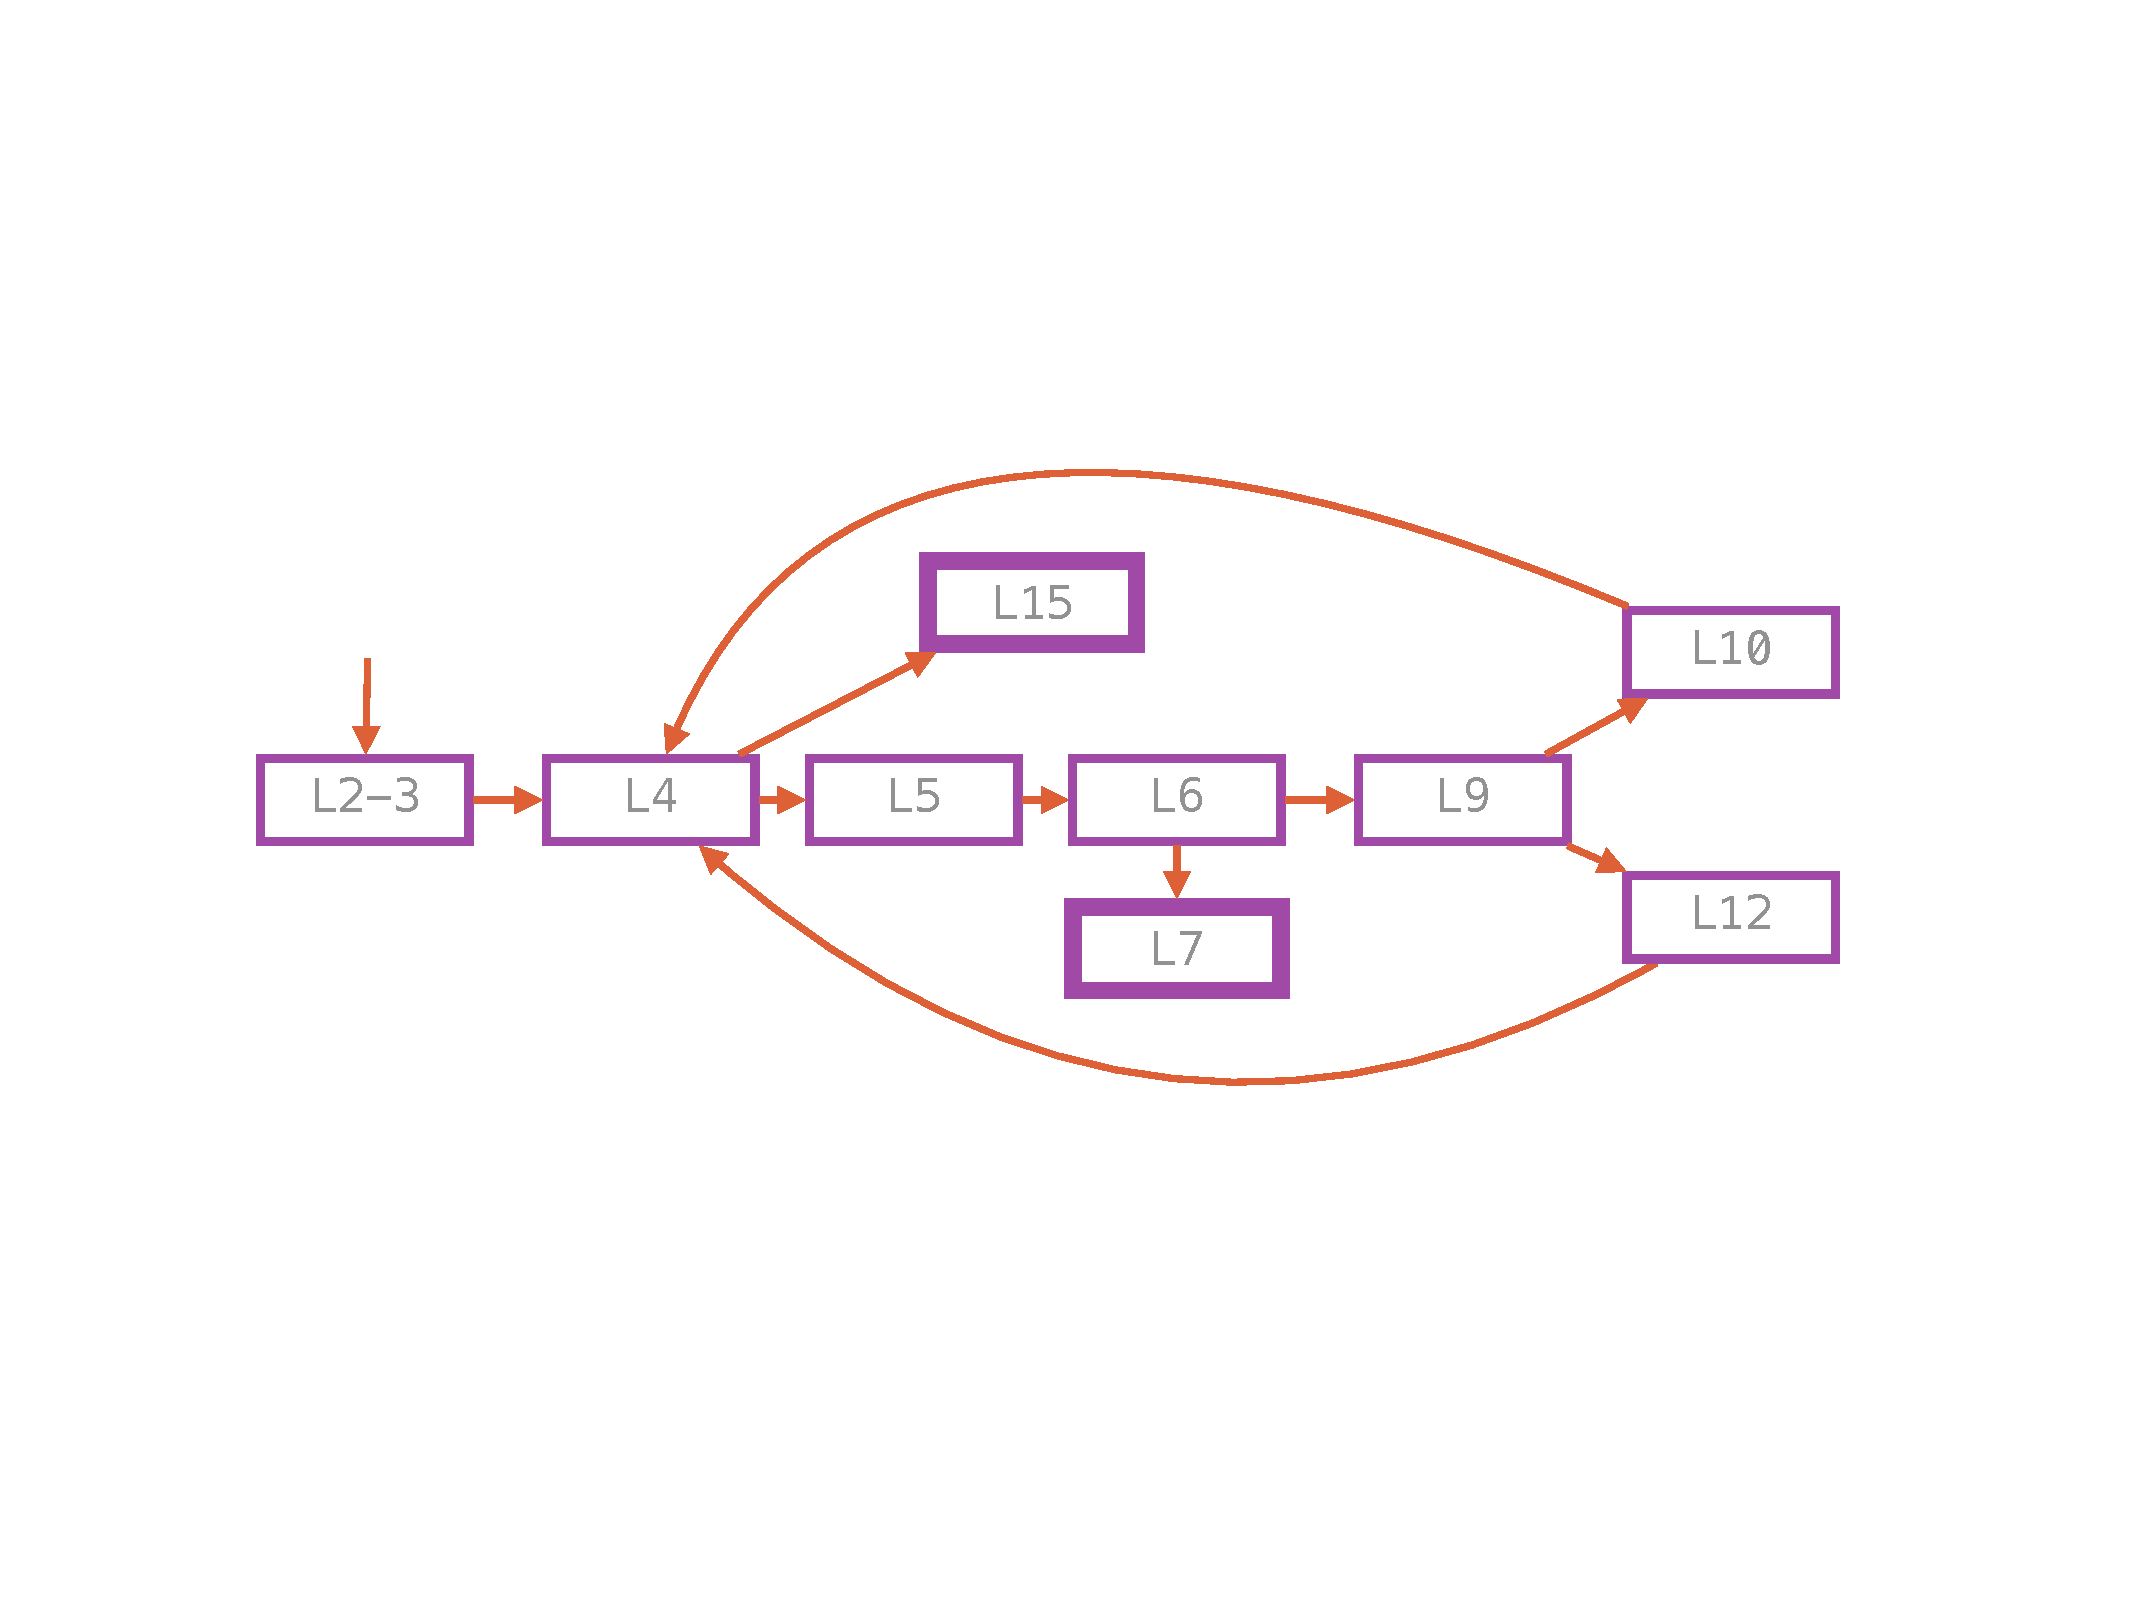
\includegraphics[width=7cm]{../midterm/figures/sample-midterm-binary-search-cfg.pdf}
  \end{solution}

\part What is a basic block? %
  \answerspace{9} %
  \begin{solution} %
    A basic block is a sequence of consecutive statements that has one
    entry point and one exit point, with no jump to/from the middle.
  \end{solution}

\part Is there any advantage to using basic blocks as opposed to
  statements in CFGs? %
  \answerspace{9} %
  \begin{solution} %
    Yes. It creates a much more compact graph, which is more efficient
    for program analyses. %
  \end{solution}

\part Is there any disadvantage to using basic blocks as opposed to
  single statements in CFGs? %
  \answerspace{9} %
  \begin{solution} %
    For structural coverage analysis there is generally no
    disadvantage. (Other answers are also valid if well justified.)
    % Yes. It is impossible to analyze the program state between statements that are grouped into the same basic block.
  \end{solution}

\end{parts}

\newpage

\question Consider the following Java function:
  \begin{minted}{Java}
public static int indexEven(int[] x, int n) {
 // if x is null, return -1
 // otherwise return the index of the n-th even number in array x
 // so that n=1 returns the first even element, n=2 returns the second
 // *or* return -1 if there is no n-th even number in array x
  if (x == null) {
    return -1;
  }
  int count = 0;
  for (int i = 0; i < x.length; i++) {
    if (x[i] % 2 == 0) {
      if (count == n) {
        return i;
      } else {
        count++;
      }
    }
  }
  return -1;
}
\end{minted}

\begin{parts}
\part State the location(s) of the program fault and explain how
  you would fix the program. Consider only the smallest and simplest
  fix. %
  \answerspace{10} %
  \begin{solution} %
    The simplest explanation\footnote{Other answers are also valid if
      well justified.} is that the fault is on line 6-- by starting
    the \mintinline{Java}{count} at 0, this function will returns the
    $n+1$-th element of the list, since the comment at the start of
    the function indicates that the first even element of the list is
    the $1-th$ one.
  \end{solution}

\part If possible, provide an example of a test input that
  does not cause the fault to execute.  If this is not possible
  explain why.

  \answerspace{10} %
  \begin{solution} %
    If the test input is (\mintinline{Java}{x}$\mapsto$
    \mintinline{Java}{null}, \mintinline{Java}{n}$\mapsto$
    \mintinline{Java}{1}), \mintinline{Java}{indexEven} will return
    on line 6 without executing the fault.%
  \end{solution}

%\newpage

\part If possible, provide an example of a test input that causes
  the fault to execute but no error state to occur. If this is not
  possible explain why. %
  \answerspace{10} %
  \begin{solution} %
    This is not possible for the scenario described above -- the
    initial value of \mintinline{Java}{count} in the correct
    implementation of \mintinline{Java}{indexEven} is always
    \mintinline{Java}{1}!%
  \end{solution}

\part If possible, provide an example of a test input that causes
  the fault to execute, the error to occur, but no failure to
  occur. If this is not possible explain why. %
  \answerspace{10} %
  \begin{solution} %
    If the test input is (\mintinline{Java}{x}$\mapsto$
    \mintinline{Java}{[1, 3, 5]}, \mintinline{Java}{n}$\mapsto$
    \mintinline{Java}{1}), the fault is executed and the initial value
    of \mintinline{Java}{count} is erroneously set to
    \mintinline{Java}{0}, but \mintinline{Java}{indexEven} returns
    \mintinline{Java}{-1}, as expected.%
  \end{solution}

\part If possible, provide an example of a test input that causes
  the fault to execute, the failure to occur, but no error to
  occur. If this is not possible explain why. %

  \answerspace{10} %
  \begin{solution} %
    This is impossible: as described in the answer to question 1b
    above, an error state \emph{must} be encountered in order for a
    failure to be observed. %
  \end{solution}

  %\newpage

\part Describe and explain the condition that an input must satisfy
  for the error state to occur. %
  \answerspace{10} %
  \begin{solution} %
    This error state happens whenever \mintinline{Java}{x} is
    non-null.
  \end{solution}

\part Describe and explain the condition that an input must
  satisfy for the failure to occur. %
  \answerspace{10} %
  \begin{solution} %
    A failure will always occur if \mintinline{Java}{x} is non-null
    and contains \emph{at least} \mintinline{Java}{n} even elements.
  \end{solution}
\end{parts}

\newpage

\question Write below a single valid Java program with fewer than 12
  lines and 12 statements, that can not satisfy two different
  categories of coverage criteria that were discussed in class.

  \answerspace{10} %
  \begin{solution} %
    \begin{minipage}{.9\linewidth}
\begin{minted}{Java}
static void sillyButFun(){
  if(false){
    System.out.println("Hello World!");
  }
}
\end{minted}
      \end{minipage}
    \end{solution}

  \begin{parts}
  \part Identify the first coverage criterion that you selected and
    thoroughly explain why it is impossible for any test suite to
    completely satisfy that criteron for your program. %
    \answerspace{7} %
    \begin{solution} %
      A test suite can never satisfy node coverage for
      \mintinline{Java}{sillyButFun}, as line 3 is dead code and can
      never be covered. %
    \end{solution}

\part Identify the second coverage criterion that you selected and
  thoroughly explain why it is impossible for any test suite to
  completely satisfy that criteron for your program.
  \answerspace{7} %
  \begin{solution}%
    A test suite can also never satisfy edge coverage for
    \mintinline{Java}{sillyButFun}, since the \mintinline{Java}{true}
    branch of the conditional can never be taken. %
  \end{solution}
\end{parts}


\newpage
\question Consider the following control-flow graph:
  \begin{center}
  \begin{figure}[ht]
    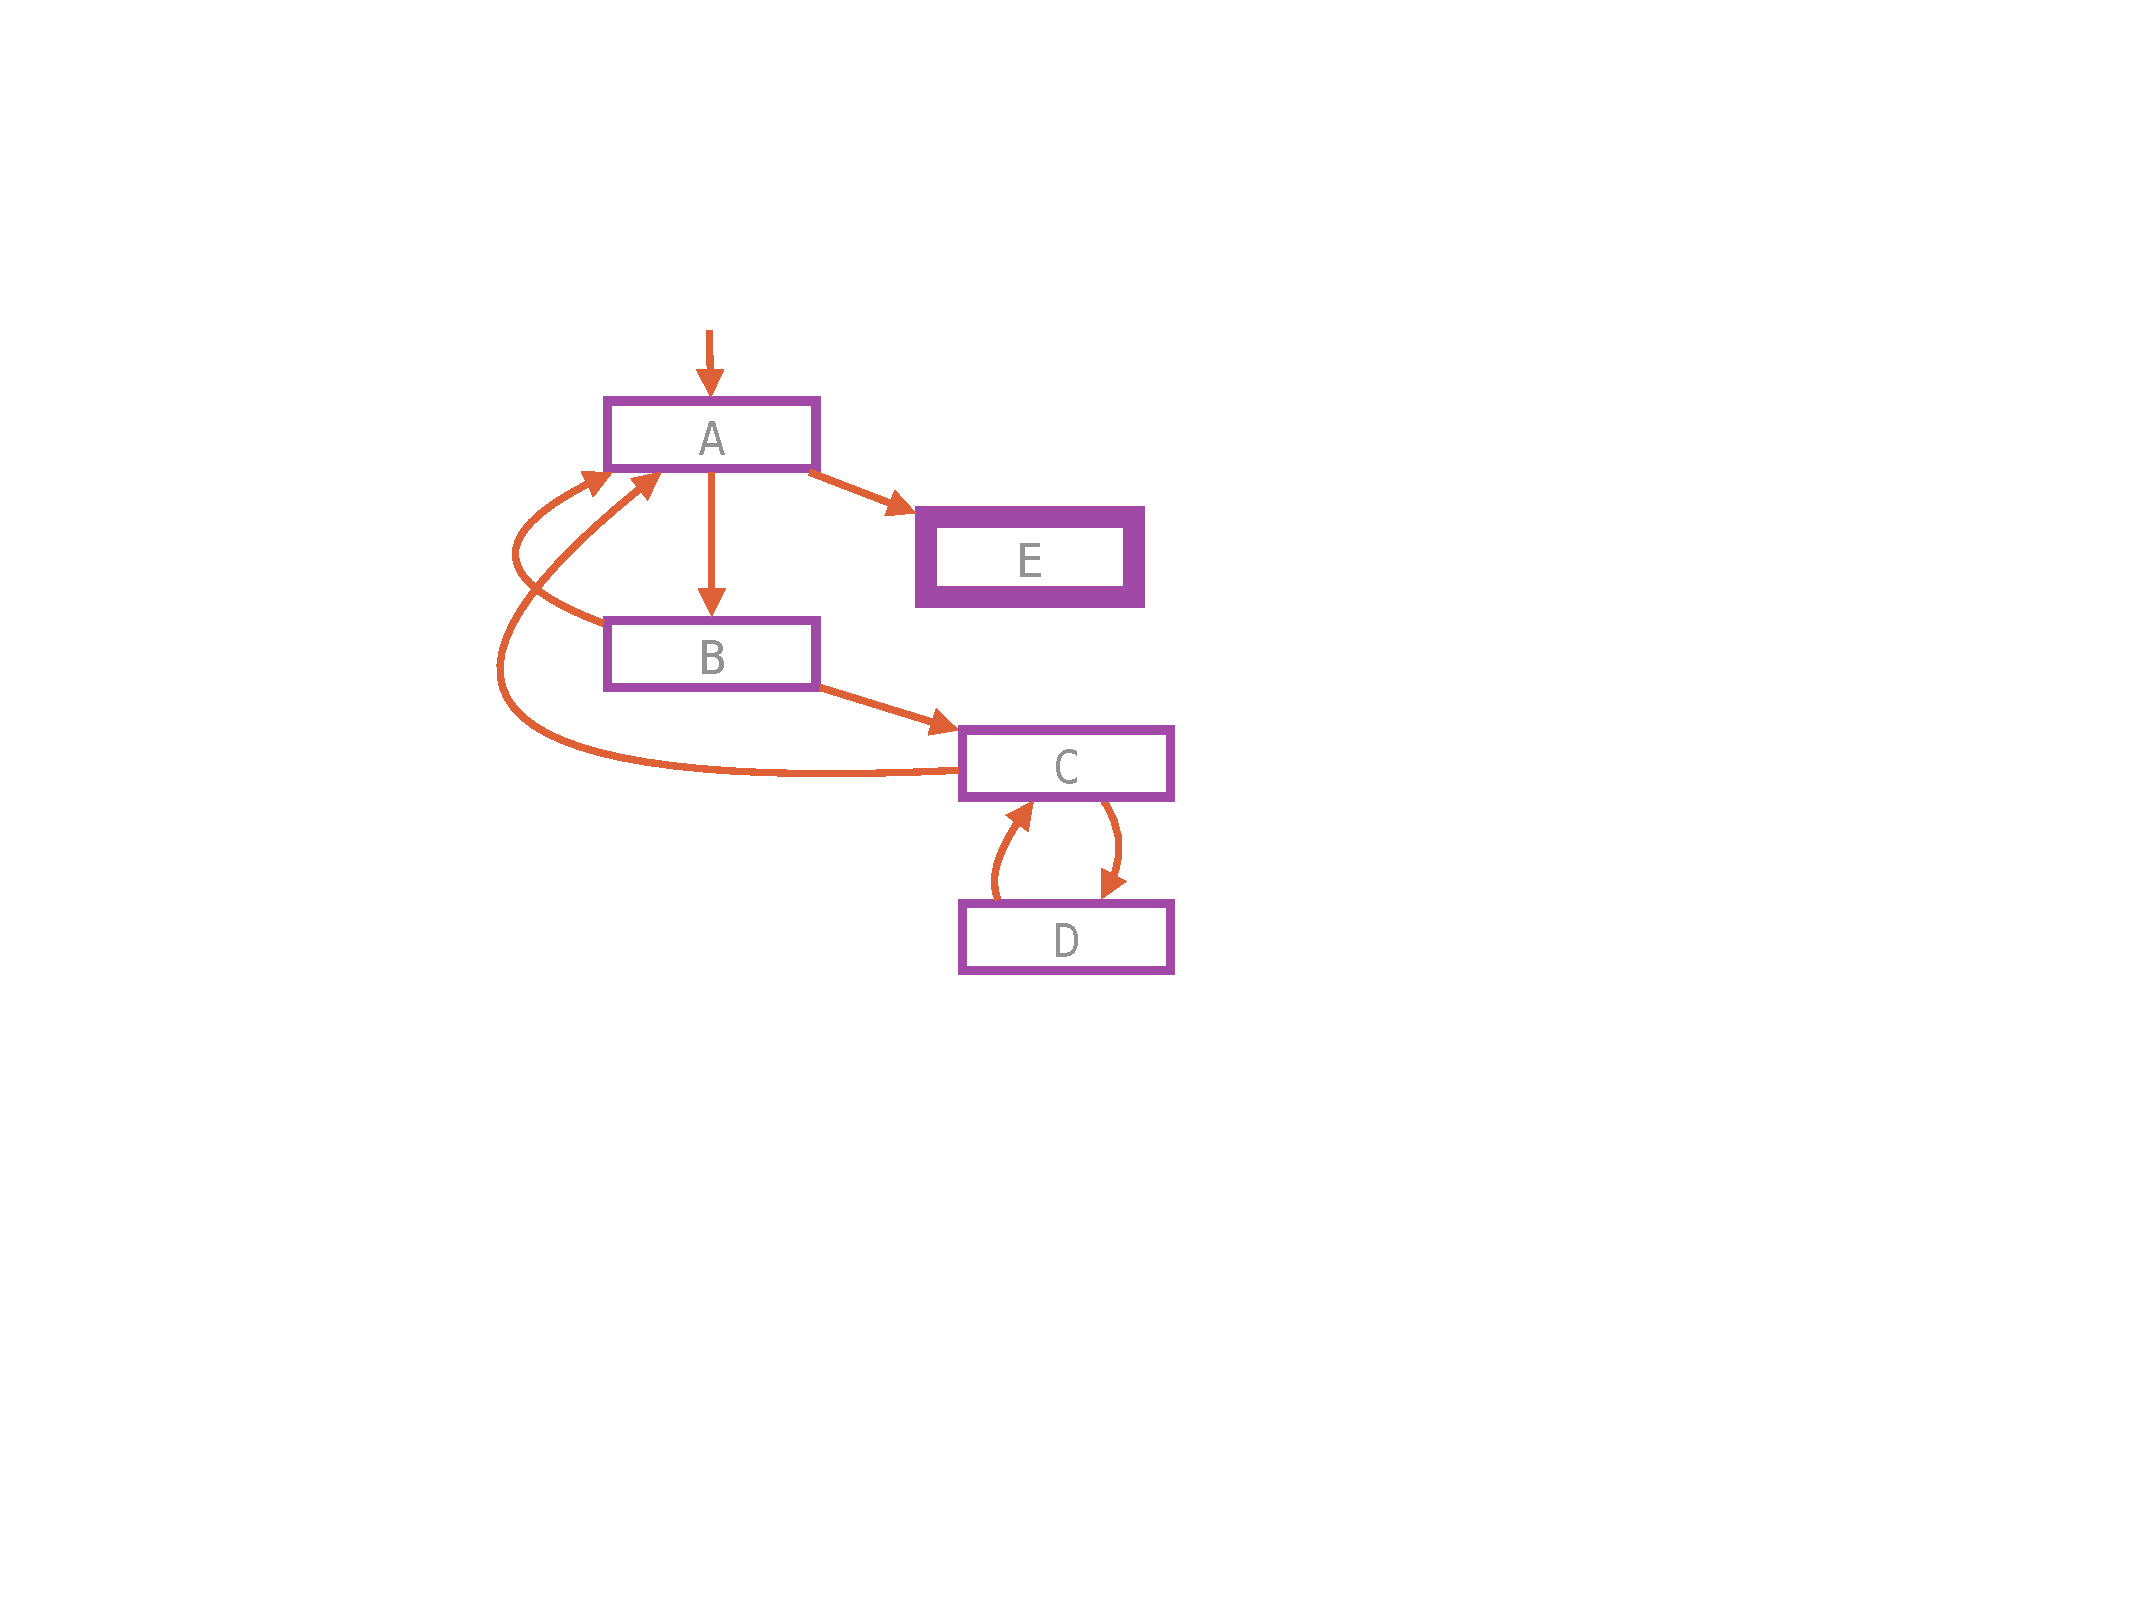
\includegraphics[width=7cm]{../midterm/figures/sample-midterm-cfg-2.pdf}
  \end{figure}
\end{center}

\begin{parts}
\part List all the simple paths in the CFG given above. %
  \answerspace{7} %
  \begin{solution} %
    \begin{itemize}
      \item[1] [A], [B], [C], [D], [E]  %
      \item[2] [A, E], [A, B], [B, A], [B, C], [C, A], [C, D], [D, C], %
      \item[3] [A, B, A], [A, B, C], [B, A, B] [B, A, E], [B, C, D],
        [B, C, A], [C, A, B], [C, A, E], [C, D, C], [D, C, A], [D, C,
        D] %
      \item[4] [A, B, C, D], [A, B, C, A], [B, C, A, B], [B, C, A, E], [C, A, B, C], [D, C, A, E],
        [D, C, A, B] % \\
      \end{itemize}
  \end{solution}

\part List three test paths in the CFG given above. %
  \answerspace{7} %
  \begin{solution} %
    The test paths must start at node A and end at node E. Note that
    there is exactly one simple test path: [A, E]. Once you allow for
    the possibility of repeated nodes, however, the world is your
    oyster: [A, B, A, E], [A, B, C, D, C, A, E], etc.
    %
  \end{solution}

\part List all the prime paths in the CFG given above. %
  \answerspace{7} %
  \begin{solution} %
    Recall that a prime path is a simple path that does not appear as
    a proper subpath of any other prime path.
    [A , B , A],
    [B, A, B],
    [B , A , E],
    [C , D , C],
    [D, C, D]
    [A , B , C , A],
    [A , B , C , D],
    [B , C , A , B],
    [B , C , A , E],
    [C, A, B, C],
    [D , C , A , B],
    [D , C , A , E]
  \end{solution}

  \newpage
\part Write an example of a syntactically valid Java function
  that generates the control-flow graph above. If this is not
  possible, explain why. %
  \answerspace{23} %
  \begin{solution}
    Here is one possible solution:
    \begin{minted}{Java}
static int sillyAndAlsoFun(int a) {
  while (a <= 52){    // A
    if (a < 53) { // B
      while (a < 53) { // C
        a += 1;         // D
      }
    }
  }
  return a;             // E
}
\end{minted}
  \end{solution}

  \part Provide test inputs that would generate the test paths
    you identified in 6a (or state they are infeasible).
    \answerspace{15}
    \begin{solution}
      \begin{itemize}
      \item [] \textbf{[A, E]}: (\mintinline{Java}{a}$\mapsto$
        \mintinline{Java}{53}, \mintinline{Java}{b}$\mapsto$ \mintinline{Java}{0}
      \item [] \textbf{[A, B, A, E]}: infeasible path
      \item [] \textbf{[A, B, C, D, C, A, E]}: \mintinline{Java}{a}$\mapsto$ \mintinline{Java}{52}
      \end{itemize}
    \end{solution}
  \end{parts}

\newpage
\question Consider the following control-flow graph annotated with
  def-use information. Unless otherwise noted, assume $def(l) =
  \emptyset$ and $use(l) = \emptyset$.
  \begin{figure}[ht]
    \begin{center}
      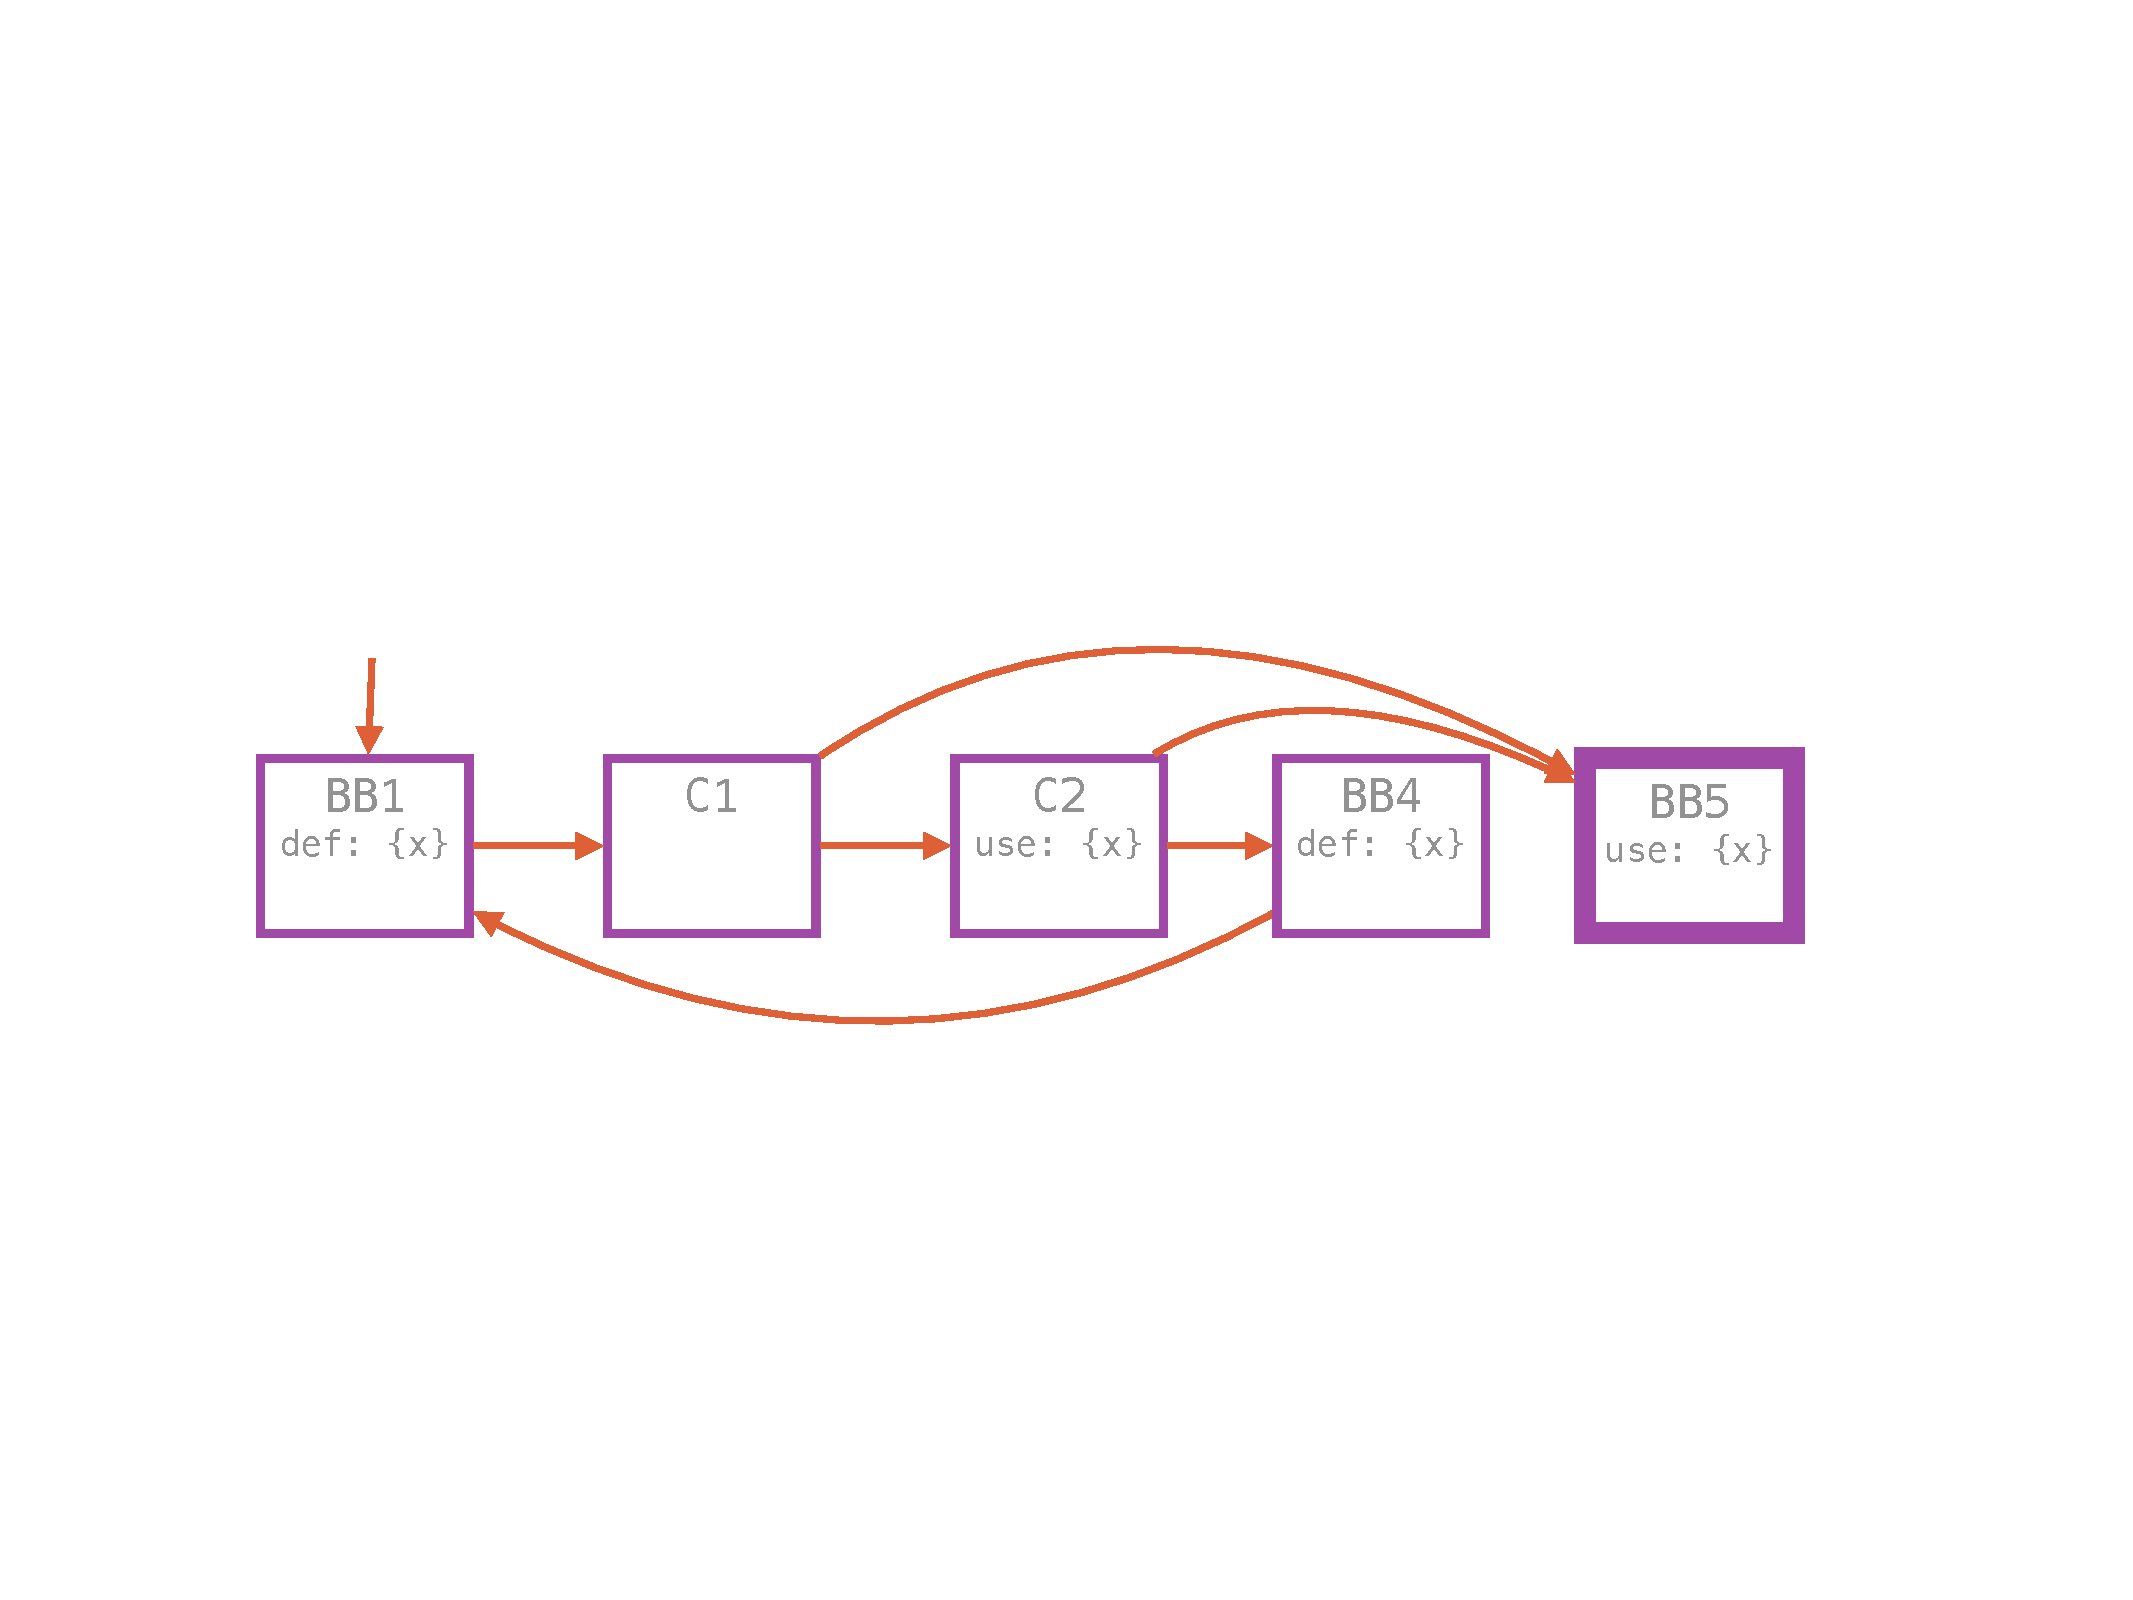
\includegraphics[width=.5\linewidth]{../midterm/figures/sample-midterm-cfg}
    \end{center}
\end{figure}


\begin{parts}
    \part List the test requirement set of all-defs coverage with respect to \mintinline{Java}{x}.
    \answerspace{12}
    \begin{solution}
      The test set includes a test case corresponding to one of the
      following paths: [0, 1, 2] or [0, 1, 5].
    \end{solution}

    \part List the test requirement set of all-uses coverage with respect to \mintinline{Java}{x}.
    \answerspace{12}
    \begin{solution}
      The test set includes a test case corresponding to each of the
      following paths: [0, 1, 2] and either [0, 1, 5] or [0, 1, 2, 5].
      % Accept answer with just:
      % - TR = {[0, 1, 2], [0, 1, 4]}    OR
      % - TR = {[0, 1, 2], [0, 1, 2, 4]}
    \end{solution}

    \part List the test requirement set of all-du-paths coverage with respect to \mintinline{Java}{x}.
    \answerspace{12}
    \begin{solution}
      The test set includes a test case corresponding to each of the
      following paths: [0, 1, 2],[0, 1, 5], and [0, 1, 2, 5].
\end{solution}
\end{parts}

\question A tester defined three characteristics for the input
  parameter car: \textbf{Where Made}, \textbf{Energy Source}, and
  \textbf{Size}. The following partitioning for these characteristics
  has (at least) two mistakes. How would you correct them?

  \begin{center}
  \begin{tabular}{|c|c|c|}
    \hline
    \multicolumn{3}{|c|}{\textbf{Where Made}} \\\hline
    North America & Europe & Asia \\\hline
    \multicolumn{3}{|c|}{\textbf{Energy Source}} \\\hline
    gas & electric & hybrid \\\hline
    \multicolumn{3}{|c|}{\textbf{Size}}\\\hline
    2-door & 4-door & hatch back\\\hline
  \end{tabular}
\end{center}
\answerspace{15}
\begin{solution}
  Some potential mistakes:
  \begin{itemize}
  \item The ``Size'' describes the number of doors, as opposed to
    'compact', 'full-size', etc. and is thus arguably incomplete. More
    importantly, the ``Size'' categories are not mutually exclusive:
    it is possible to have a hatchback car with 4-doors, for
    example. The solution is to divy this up into proper, distinct
    size categories: [compact | mid-size | full-size | SUV/truck]
  \item The ``Where Made'' category is similarly incomplete: Brazil is
    a major car manufacturer, and Australia has been known to produce
    cars. One solution is to add additional categories, e.g.,
    [North America | Asia | Europe | South America | Other]
  \end{itemize}
\end{solution}

\newpage

\question Explain how the coverage-guided fuzzers discussed in class work.
\answerspace{20}
\begin{solution} Grey-box fuzzers randomly test a program by
  iteratively generate new tests by mutating a corpus of test inputs
  derived from an initial set of test. They insert lightweight
  instrumentation to gather coverage feedback from each test execution
  to identify if a new test has covered a new node or branch, and use
  this information to update the corpus of test inputs and when
  generating the next test input.
  \end{solution}

  \newpage

\question
  Provide a simple example of a program with a data race, where the
  lockset algorithm can help identify the problem. Provide and explain
  the results of the lockset algorithm on this program. %
  \answerspace{20} %
  \begin{solution}
    \begin{minted}{Java}
int balance = 0;
Lock lockA = new Lock();
Lock lockB = new Lock();

// Thread 1
void deposit() {
    lockA.lock();
    balance = balance + 100;
    lockA.unlock();
}

// Thread 2
void withdraw() {
    lockB.lock();
    balance = balance - 50;
    lockB.unlock();
  }
\end{minted}
    Suppose the test executes the first thread to completion, and then
    the second thread. The initial lockset for \mintinline{Java}{balance} will be \{A, B\},
    after executing the first thread, it will be \{A\}, and after
    executing the second, it will be \{ \}.


\end{solution}

\question Provide a simple example of a program without a
  problematic data race, where the lockset algorithm will nevertheless
  flag a potential data race for the user. Provide and explain the
  results of the lockset algorithm on this program, and argue why this
  is a false positive.

  \answerspace{20}%
  \begin{solution}
    \begin{minted}{Java}
int balance = 0;
Lock lockA = new Lock();

// Thread 1 - This thread is always run before the other two
void init() {
    balance = 100;
}

// Thread 2
void deposit() {
    lockA.lock();
    balance = balance + 50;
    lockA.unlock();
}

// Thread 3
void withdraw() {
    lockA.lock();
    balance = balance - 25;
    lockA.unlock();
}
\end{minted}

    Here, the lockset algorithm will identify the first write to
    \mintinline{Java}{balance} as not being protected by any locks,
    and thus report a potential data race after \emph{every} test
    execution. This is okay however -- this use of
    \mintinline{Java}{balance} is actually protected by the control
    flow structure of the client program, which ensures that there can
    never be any concurrent accesses of  the variable while the first
    thread is running.
  \end{solution}




% \newpage
% \question[5] Describe two approaches to determine what are the properties of good bug reports. Explain how you would implement each.
% \answerspace{16}
% \begin{solution}Examples: (a) conducting developer surveys and (b) studying the properties of bug reports in bug repositories.}


\newpage



\if 0 %%%%%%%%%%%%%%%%%%%%%%%%%%%%%%%%%%%%%%%%%
	\question[10]
	\answerspace{30}
	\begin{solution}}

	\question
	\begin{parts}
		\part[6]
		\answerspace{20}
		\begin{solution}}

		\part[2]
		\answerspace{10}
		\begin{solution}
                \end{answer}

	\end{parts}
\fi %%%%%%%%%%%%%%%%%%%%%%%%%%%%%%%%%%%%%%%%%

	\newpage
	\begin{center}
		[EMPTY PAGE 1]
	\end{center}

	\newpage
	\begin{center}
		[EMPTY PAGE 2]
	\end{center}

\end{questions}





\end{document}
